\chapter{Macrosegregation with liquid metal motion}
\begin{nolinkcolors} 
\minitoc
\end{nolinkcolors}
\newpage
%
%
\section{Introduction}
Fluid flow is an important part, if not the most important, in understanding the evolution of a system
undergoing phase change and chemical segregation. It is attributed to the convective transport in fluids
where the variations time scale is much smaller than the remaining physics that are characterised by
smoother variations. To understand how fluid motion contributes to the heat and mass transfer, we have 
swiftly presented the momentum conservation equation in a solidifying liquid, \cref{eq:Navier-Stokes2}.
In this chapter, we will first give quick overview of the numerical treatment of this system of 
Navier-Stokes equations, then comment on some computational aspects such as the choice of a suitable time step and
the conditions that impose minimum and maximum bounds on both time step and mesh size.
%
%%-----------------
%
\section{Formulation stability}
A wide array of numerical methods can be used to solve systems like \cref{eq:Navier-Stokes2}. 
When speaking about Navier-Stokes equations, the choice can be narrowed to two famous
approaches with some similarities: stable mixed finite element method and \textbf{V}ariational \textbf{M}utli\textbf{S}cale (VMS) method.
When two finite element spaces are introduced (e.g. one for velocity and another for pressure), 
the essential \emph{inf-sup} condition (also known as stability condition) determined by \citet{babuska_error-bounds_1971} and \citet{brezzi_existence_1974} 
should be fulfilled. It states that the formulation is not well-posed if the both spaces have the same interpolation 
order. For instance, a P1/P1 element (i.e. P1 for velocity / P1 for pressure) cannot guarantee the stability of the Navier-Stokes solution since
velocity and pressure are both linearly interpolated at the simplex vertices.
However, the major difference between the previously mentioned formulations is the way in which the inf-sup condition is accounted for.
Stable mixed finite elements are stable because they directly respond to the stability condition by enriching the velocity space, 
hence they fall under the category of Satisfying Babuška-Brezzi (SBB) methods. In contrast, methods like VMS belong to the
Circumventing Babuška-Brezzi (CBB) category \citep{barbosa_finite_1991}.
CBB methods rely on equal-order interpolations with additional stabilisation that circumvents the need to satisfy the stability condition.
Further details about both formulation types are given in the next subsections.
%
\subsection{Stable mixed finite elements}
First introduced by \citet{arnold_stable_1984}, the MINI element is the key ingredient of this approach.
This type of element introduces an additional degree of freedom for the velocity field while keeping a linear
interpolation for the pressure field, thus satisfying the Babuška-Brezzi condition with a richer velocity space.
The additional degree, known as the \emph{bubble} function, vanishes on the element's boundary.
We may therefore speak of a P1+/P1 finite element in a velocity-pressure formulation. 
This stable formulation has been the de facto standard for solving fluid 
and solid mechanics for many years at CEMEF.
%
%-----------------------
\begin{figureth}
{0.75}
{Chapter3/Graphics/minielement/minielement.pdf}
{Schematic of 2D and 3D stable P1+/P1 finite elements, respectively triangle and tetrahedron, with velocity and pressure fields interpolation order.
The dots represent the nodes while the squares represent the bubbles.}
\label{fig:minielement}
\end{figureth}
%--------------------------------------------------------
%
\subsection{Variational multiscale (VMS)}
As the name indicates, this approach considers two scales of phenomena: the coarse and fine scales. Applied to a velocity-pressure
formulation, these fields are decomposed according to these scales as follows:
%----------------
\begin{align}
\label{eq:vms_multiscale_v}
 &\vit = \vit_h + \tilde{\vl} \\ 
\label{eq:vms_multiscale_p}
 &p = p_h + \tilde{p}
\end{align}
%----------------
where $\vit_h$ and $p_h$ are the coarse scale velocity and pressure discretised on the finite element mesh (hence the subscript $h$), 
while the remaining terms represent the fine scale velocity and pressure that cannot be captured at the scale of the FE grid. Instead 
of defining a finer grid to model the effect of these terms, one can solve the fine scale equations obtained once \cref{eq:vms_multiscale_v,eq:vms_multiscale_p}
are injected in \cref{eq:Navier-Stokes2} then use the output in the coarse scale equations. Further technical details about the method and the equations are
found in the PhD work of \citet{hachem_stabilized_2009}. The added value of the VMS method is the time gain that we get by incorporating the effect of the fine scale into the 
coarse scale physics without discretising on a finer grid, while maintaining the ability to predict localised fluid motion such as small vortices.
%
%%-----------------
%
\section{VMS solver}
In the present thesis, we chose to solve the fluid momentum conservation using the VMS approach. The VMS solver developed 
by \citet{hachem_stabilized_2010} is a convenience choice to solve Navier-Stokes with Darcy terms while at the same time 
have convection stablisation terms, such as the well known Streamline Upwind Petrov-Galerkin (SUPG) and Shock Capturing Petrov-Galerkin (SCPG)
stabilisation techniques for convection-dominated problems.
%\subsection{Variational form}
\subsection{Variational formulation}
%
\subsection{CFL condition}
%
\subsection{Integration order}
%
Using P1 linear elements implies a P2 integration ? what are the advantages (time) and limitations ?

%-------------------------------------------------------------
\section{Application to multicomponent alloys}
In the previous chapter, we have considered a static melt upon solidification of multicomponent alloy. 
The artificial consideration of a still flow is dropped in this chapter, hence taking into account macrosegregation 
caused by fluid motion, using realistic values of the expansion coefficients given in \cref{table:ternary_data_case}.
In the real conditions, the melt is in constant motion and knowing that the carbon and chromium solutes have lightening effects on the liquid 
at nominal composition, the density inversion resulting from the composition gradient in the interdendritic 
liquid, may cause flow instability (segregation plumes) at the solidification front. While the selected alloy 
is a steel, this application is also representative of directional cooling in a single crystal casting, e.g. 
for nickel-base superalloys \citep{beckermann_development_2000}. Solidification of this class of alloys is carefully
controlled so as to prevent any freckle-type defect to exist in the as-cast state.
In this section, we consider the same simulation parameters defined in \cref{table:ternary_data_case} as well the geometry and thermal boundary conditions
previously defined in \cref{fig:mutlicomponent_geobc}. Moreover, we solve the liquid momentum conservation equation, with non-slip boundary conditions
on all external sides of the cylinder.
%
%=====================================BIG LANDSCAPE FIGURE =====================================
\begin{landscape}
\begin{figureth}
{1.15}
{Chapter3/Graphics/multicomponent/planche_macroseg.pdf}
{: Upward solidification of a cylinder rod  at 3 stages showing the metallurgical consequences 
of macrosegregation \tern{Fe}{2}{C}{30}{Cr}. The left columns show the average 
composition and temperature distribution, while the right columns show the phase fractions.}
\label{fig:planche_withmacroseg}
%\thispagestyle{headings}
\end{figureth}
\end{landscape}
%=====================================BIG LANDSCAPE FIGURE =====================================
%
\subsection{Results}
Solidification starts at 407 s when the cylinder’s bottom base temperature 
reaches the liquidus temperature of the alloy. 
In fact, the solidification onset is the same as in the pure diffusion case in \cref{fig:planche_nomacroseg}, 
since the average composition remains unchanged for an entirely liquid domain (assuming an initially infinite 
solute mixing in the melt). As shown in \cref{fig:planche_withmacroseg} at 600 s, the first solid phase to form 
remains ferrite. We can also see solute-rich channels forming in the mushy zone and solute 
plumes rising in the melt above the mushy zone due to a subsequent upward flow. It is actually 
caused by the thermosolutal buoyancy force created by the carbon and chromium solutes. Such 
phenomenon could delay solidification inside liquid-rich channels and results in a freckling 
defect \citep{felicelli_simulation_1991} on the surface of the cylinder as well as inside, as shown later in this section. 
As solidification proceeds, the liquid becomes more enriched with solute and the peritectic 
reaction forming the austenite phase is reached. However, for very large enriched melt, it can 
also be observed that primary solidification proceeds with the austenite phase rather than the 
ferrite phase. The carbide phase can also form with the austenite phase at some locations. These 
observations correspond to a simulation time of \num{2000} s in \cref{fig:planche_withmacroseg}. Solidification ends at 
around \num{2475} s, the last liquid solidifying at the cylinder’s top surface, where the average composition 
reaches a maximum of \tern{Fe}{2.151}{C}{30.633}{Cr}, i.e. a relative positive macrosegregation, 
$\brac{\wi-\wi_0}/\wi_0$, of 7.5\% for carbon and 2.1\% for chromium. The fact that the maximum average 
composition is observed at the top, is verified in \cref{fig:final_interior_ZZ_FF} which shows the composition map in a 2D 
vertical slice through the longitudinal axis of the cylinder. We can also see it in \cref{fig:final_segregation_ZZ_FF} where the 
relative composition profile are plotted at the end of the cooling process along the longitudinal cylinder 
axis Z-Z’ and along the axis of the segregated channel, F-F’. The negative segregation up to 1 cm from the chill corresponds 
to the solute depletion caused by the first solid formation. The subsequent solidification enriches further the 
liquid; hence the solid composition also increases. The composition evolution trend for both solutes is similar: 
an overall rise until positive segregation is achieved above \SI{5}{\centi\metre} from the chill. The positive macrosegregation 
intensifies when the profile is chosen at the center of the segregated channel, negative segregation then becoming less pronounced.
%
%-----------------
\begin{figure}[htbp]
\centering
   %------------
  \begin{subfigure}[t]{0.4\textwidth}
    \centering
	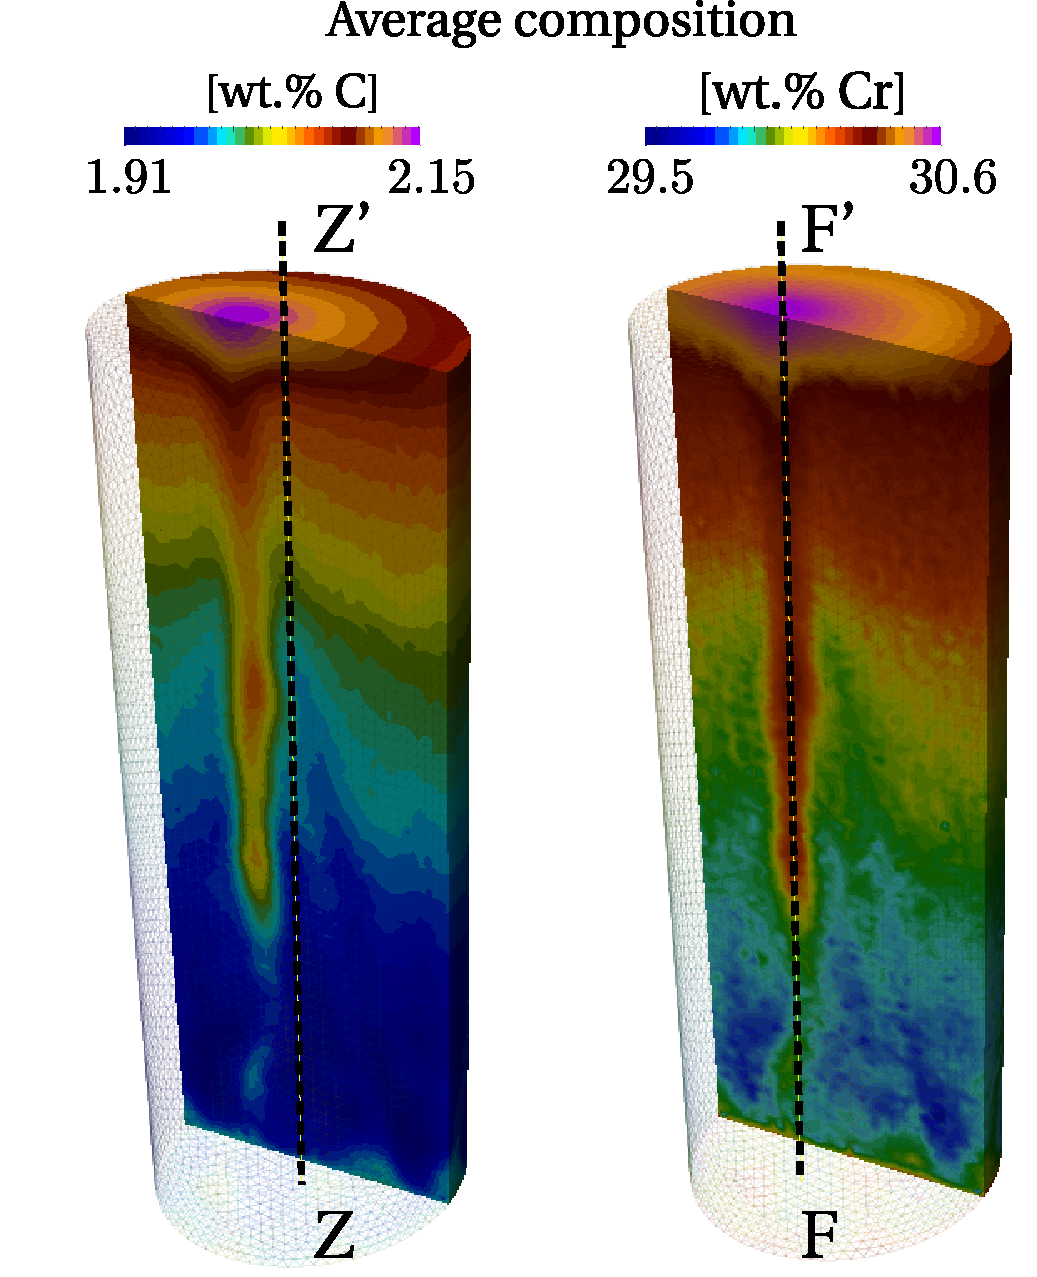
\includegraphics[width=1.0\textwidth]{Chapter3/Graphics/multicomponent/interior/final_interior_ZZ_FF.pdf}
	\caption{}
    \label{fig:final_interior_ZZ_FF}
  \end{subfigure}
  %------------------------------
	\hfill  
   %------------------------------
  \begin{subfigure}[t]{0.55\textwidth}
    \centering
	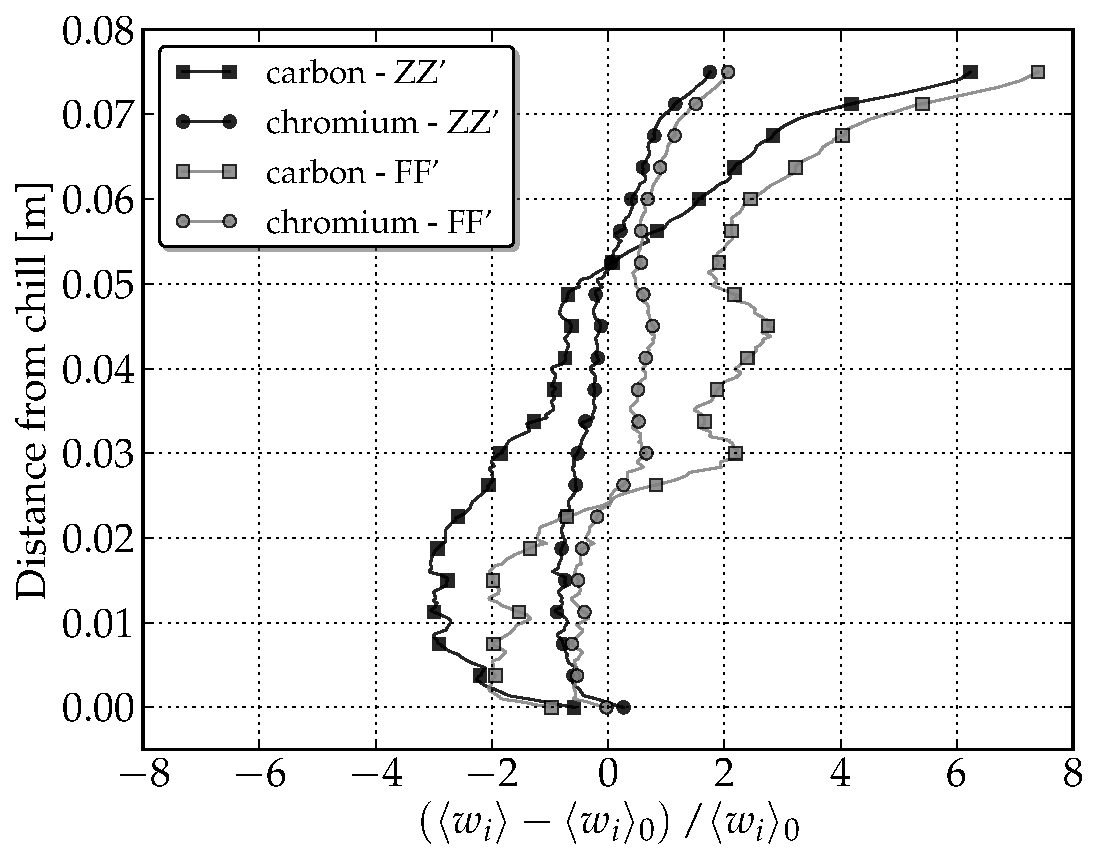
\includegraphics[width=1.0\textwidth]{Chapter3/Graphics/multicomponent/interior/final_segregation_ZZ_FF.pdf}
	\caption{}
    \label{fig:final_segregation_ZZ_FF}
  \end{subfigure}
   %------------
\caption{(a) average composition map on a vertical section inside the sample, with
 (b) relative macrosegregation profiles on the vertical revolution axis.} 
\label{fig:final_ZZ_FF}
\end{figure}
%------------------
%
Beyond \num{2475} seconds, no variations of the average composition maps are observed since solute diffusion 
in the solid phases is neglected. Nonetheless, as temperature decreases, solid-state transformations are 
still possible as for the case with no macrosegregation. The formation of a cementite phase begins at the 
cylinder base at \num{8843} s with a temperature of \SI{496.9}{\udegC}. At about \num{9293} s, the isotherm \SI{488.5}{\udegC} reaches the 
top surface. This temperature value is the local cementite solvus temperature. The difference in the solvus 
temperature between the bottom and top surfaces is due macrosegregation. Macrosegregation also explains the 
variation in the cementite content. The solid state transformation ends shortly before \num{10500} s. The influence of the solidification process is clear on 
the final macrosegregation pattern, hence the final phase distribution. This is better illustrated by drawing the time evolution of phase fractions at the 
center of the bottom and top surfaces of the cylinder in \cref{fig:tp_macroseg_influence}. With no macrosegregation, in 
\cref{fig:tp_nomacroseg}, the final distribution of the phases is the same at time \num{12000} s, while with macrosegregation, 
in \cref{fig:tp_withmacroseg}, variations of the cementite and ferrite are revealed. 
The segregated channels inside the cylinder and on the boundary, are often termed "freckles" when they consist of visible equiaxed grains \citep{copley_origin_1970}.
This defect is marked by a noticeable gradient of composition and phase fractions, possibly changing the mechanical 
properties in the channels, hence the overall mechanical behaviour of the alloy . The coupling of the Tsolver with 
thermodynamic tabulations is thus demonstrated. It shows the ability to predict complex solidification paths, even if 
only at equilibrium. As for the computation time, the Tsolver resolution performed better: 500 seconds of solidification 
required 6 hours 14 minutes compared to 8 hours 6 minutes spent by the enthalpy resolution with 12 cores on the same machine. 
The gain factor is about 22\%.
%
%-----------------
\begin{figure}[htbp]
\centering
   %------------
  \begin{subfigure}[t]{0.6\textwidth}
    \centering
	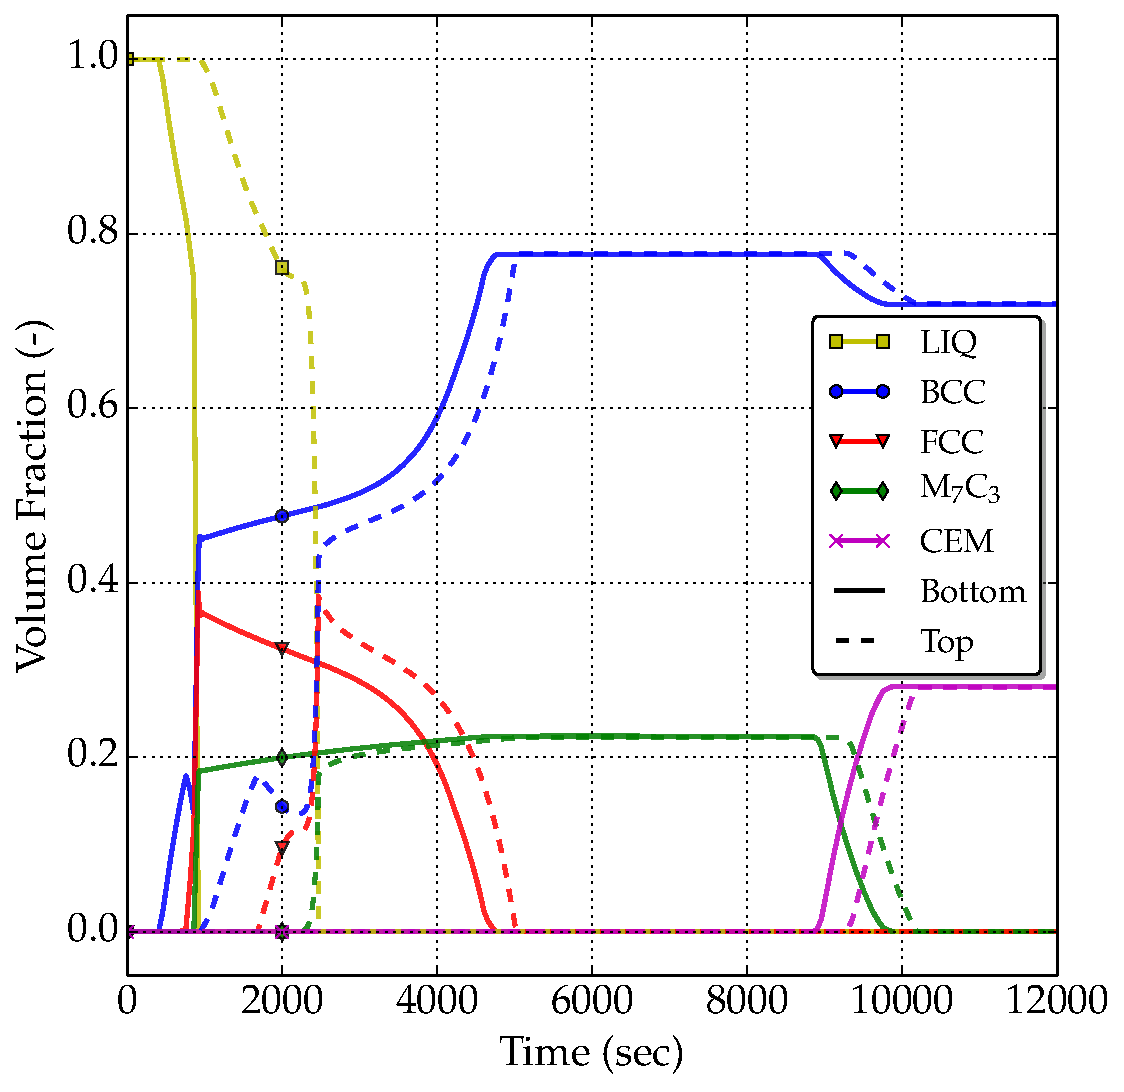
\includegraphics[width=\textwidth]{Chapter3/Graphics/multicomponent/transformationpath/TP_nomacro.pdf}
	\caption{}
    \label{fig:tp_nomacroseg}
  \end{subfigure}
  %------------------------------
  \vskip\baselineskip
  %------------------------------
  \begin{subfigure}[t]{0.6\textwidth}
    \centering
	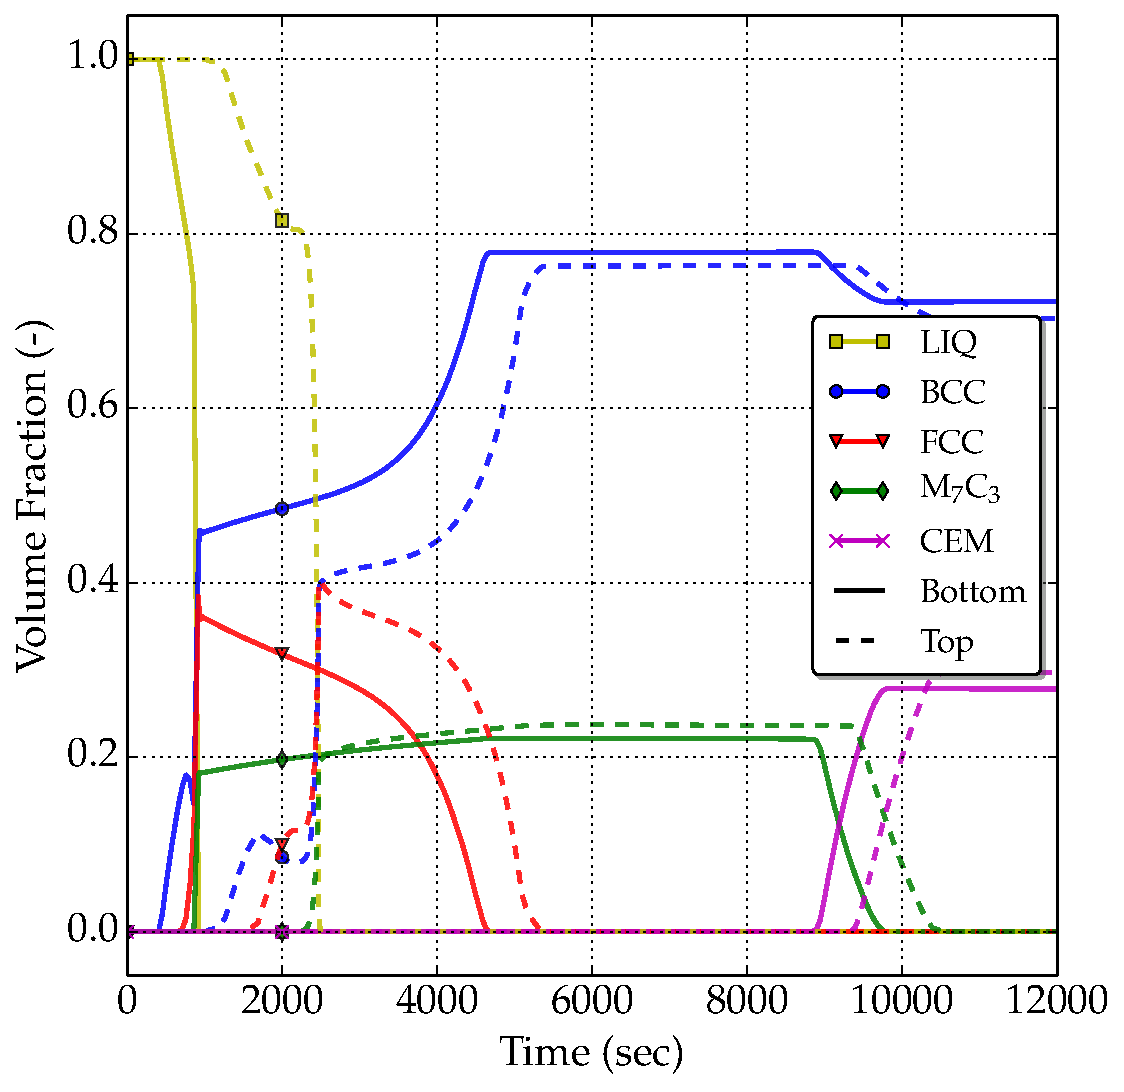
\includegraphics[width=\textwidth]{Chapter3/Graphics/multicomponent/transformationpath/TP_macro.pdf}
	\caption{}
    \label{fig:tp_withmacroseg}
  \end{subfigure}
   %------------
\caption{History of phase fraction (a) without macrosegregation and (b) with 
macrosegregation at the center of the (plain) bottom and (dashed) top surfaces 
of the cylinder surfaces, extracted from simulations displayed in (a) \cref{fig:planche_nomacroseg}
and (b) \cref{fig:planche_withmacroseg}.} 
\label{fig:tp_macroseg_influence}
\end{figure}
%------------------
%
\section{Macroscopic prediction of channel segregates}
%\comment{I should maybe mention that a constant gradient in the coming simulation is a one big difference compared to the previous FeCrC simulation}
%--------------------------
\subsection{Introduction}
\label{sec:intro_freckle}
We have seen in the previous multicomponent solidification test case, a formation of segregated channels in the cylinder. 
This defect manifests itself as a composition inhomogeneity that is highly non-isotropic. A typical description of its 
morphology would consider a channel with a diameter proportional to few primary dendrite arm spacing and a length that 
could vary from millimeters to centimeters. These “worm”-like shapes could form during directional solidification of cast 
parts designed for engine applications, particularly in Nickel-base superalloys \citep{giamei_nature_1970,beckermann_development_2000,
genereux_characterization_2000,schneider_modeling_1997}. In the latter situation, the channels are filled with a chain of small equiaxed 
crystals, thus referring to the term “freckle”. In large steel ingots, these channel defects are also related to A- and V-segregates   
\citep{pickering_macrosegregation_2013}. 

Considering a binary alloy with a partition coefficient less than unity and having a negative liquidus slope, 
freckles may form by the following mechanisms: i) solute partitioning occurs at the scale of dendrite arms and 
solute is rejected in the melt, ii) local composition gradients are intensified resulting in an increase of the 
solutal buoyancy force in the mushy zone, iii) solute-rich pools are formed, causing segregation chimneys and convective plumes in the melt, 
iv) which lead to partial remelting and transport of dendrites, continuous solute feeding and locally delayed solidification,
and finally v) accumulation of fragments and/or equiaxed crystals in the chimneys before the end of solidification.

Because it is of prime importance to control the occurrence of channel segregation, several attempts have been made 
from the late 1960’s \citep{flemings_macrosegregation:_1967, flemings_macrosegregation:_1968-1,flemings_macrosegregation:_1968} 
to the early 2000’s \citep{ramirez_evaluation_2003} to understand it and characterise it by deriving freckling criteria. 
These studies are summarized in \citep{auburtin_determination_1998}. One of the reasons for only considering freckling criteria 
is that direct realistic simulations of the formation of freckles in a casting geometry are still difficult. 
Indeed, experimental observations show that it requires a satisfying description of the microstructure together 
with the 3D convective flow controlled by the cooling conditions of the complete cast part \citep{shevchenko_chimney_2013}. 
Such information is not accessible yet. Only simulations in representative simple cuboid or cylindrical domains are 
usually achieved \citep{felicelli_simulation_1991,felicelli_modeling_1998,kohler_peritectic_2008,guo_three-dimensional_2003}, 
except when considering small volume casting \citep{desbiolles_micro-macrosegregation_2003}. 
They are usually limited to unstable thermosolutal convection without or with 
little regard to the microstructural features. Considering the spatial resolution of the defect, being for example of the 
order of the primary dendrite arm spacing, a fluid flow computation in the 3D casting part is also very demanding and not 
common in the literature. 
Among  other criteria, the dimensionless Rayleigh number has been identified as a good indicator 
for  the occurrence of segregation channels or a subsequent freckle defect. The dependence of freckling tendency on the 
Rayleigh number has been studied numerically 
and compared to experimental observations, as done by \citep{ramirez_evaluation_2003}.
%--------------------------
\subsection{Experimental work} 
\label{sec:freckle_exp}
An interesting experimental work on directional solidification of \bin{In}{75}{Ga}
featuring in-situ X-ray monitoring has been recently carried out by \citet{shevchenko_chimney_2013}. 
The comparison with numerical modelling is paramount for two main reasons: firstly, the in-situ technique allows to follow solidification in real-time 
and offers visual description of the system behaviour: grain morphology, composition evolution, effect on fluid flow in the 
mushy zone and chimney initiation, as well as other modelling input data such as dendritic and eutectic nucleation undercooling; 
secondly, an indium-gallium system is more representative of metallic alloy solidification than the widely used organic systems, 
e.g. the succinonitrile-acetone mixture that exhibits alloy-like dendritic formation in its growth stage. Further information with respect 
to the experimental hardware, procedure and data analysis can be found in \citep{boden_x-ray_2008,shevchenko_chimney_2013}.
%
%-----------------
\begin{figure}[htbp]
\centering
  %------------
  \begin{subfigure}{0.5\textwidth}
    \centering
	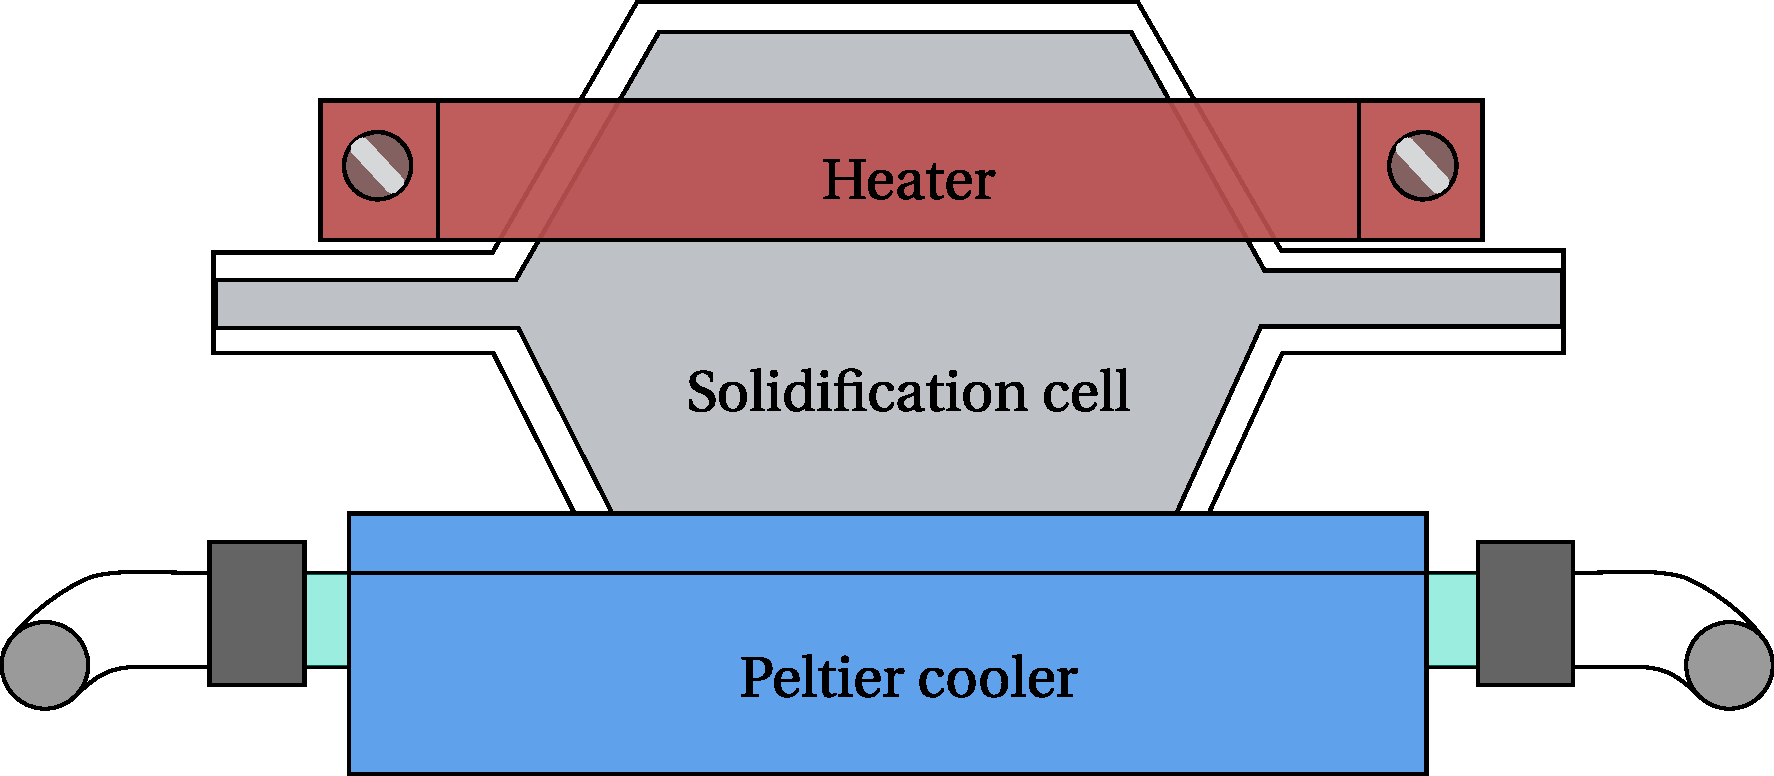
\includegraphics[height=3.5cm]{Chapter3/Graphics/freckle_exp/setup.pdf}
	\caption{}
    \label{fig:experimental_setup}
  \end{subfigure}
   %------------------------------
  %\vskip\baselineskip
  %------------------------------
  \begin{subfigure}{0.5\textwidth}
    \centering
	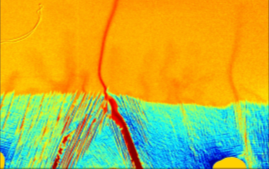
\includegraphics[height=4cm]{Chapter3/Graphics/freckle_exp/img.png}
	\caption{}
    \label{fig:experimental_img}
  \end{subfigure}
   %------------
\caption{Illustration of the benchmark experiments for in-situ observation of segregated channels
formation using X-Ray radiography with (a) a schematic of the cell and (b) a typical image 
of the microstructure formed during directional solidification of an \bin{In}{75}{Ga} alloy. Reproduced from \citep{shevchenko_chimney_2013}.} 
\label{fig:experimental_freckles}
\end{figure}
%-----------------
%
%--------------------------
\subsection{Macroscopic scale simulations}
%
\subsubsection{Configuration}
The focus of this section is on qualitative comparison between numerical simulation and the previously mentioned experiment. 
The experimental cell geometry shown in \cref{fig:freckle} is hexagonal. With adiabatic lateral sides, it results in a 
bending of the isotherm surfaces as shown in the experiment. The metallic cooling plates shown in \cref{fig:experimental_setup}
partly compensate for this effect. However, a residual horizontal component of the temperature gradient 
remains. To qualitatively replicate this effect while simplifying the cell geometry, a \SI{22 x 22 x 1}{\milli \uvolume}  
cuboid cell is considered with small cooling fluxes on its lateral vertical side surfaces computed using a constant heat transfer 
coefficient, $\hext$, and a constant environment temperature, $\Text$. Temperatures at the bottom and top surfaces, 
respectively $\Ttop$  and $\Tbottom$, are imposed in a way to maintain a constant vertical gradient, G, thus linearly 
decreasing over time with the same cooling rate R. Both square faces of the geometry, having an area of \SI{22 x 22}{\milli \uarea}, 
are adiabatic. In spite of taking cell dimensions similar to benchmark experiments presented above, the cell thickness 
is increased from \SI{150}{\micro \metre} to \SI{1}{\milli \metre}. This facilitates the computation and will later be subject to discussion. 
%
%--------------------------------
\begin{table}[htbp]
\centering
\caption{Summary of the simulations and and the corresponding parameters for the FE cases, where a purely macroscopic model is used.
Parameters are varied from (G1) low to (G2) high gradient and (L0) no, to (L1) low lateral cooling.}
\label{table:simulation_InGa_fe}
\resizebox{\columnwidth}{!}{%
{\tabulinesep=1.1mm \begin{tabu}{C{2cm} C{3cm} C{2.5cm} C{3cm} C{4.5cm}}
\tabucline[1pt]{-}
\textbf{Case} & Vertical gradient & Cooling rate & Lateral cooling & Initial temperature \\
			  &     G 			  & 	R		 & 			L \quad ($\hext$, $\Text$)	& ($T_{top}$, $T_{bottom}$) \\
 			  & [\si{\ugradT}] & [\si{\uCR}] &  [\si{\uhconvec}, \si{\udegC}] &  [\si{\udegC}]\\\tabucline[1pt]{-}
%-----------------------------
FE-G1R1L0 & G1:0.2 & R1:-0.01 & L0:(0,0) & (29.75, 25.25)  \\ 
FE-G1R1L1  & G1:0.2 & R1:-0.01 & L1:(20,0) & (29.75, 25.25)  \\ 
FE-G2R1L1  & G2:1.5 & R1:-0.01 & L1:(20,0) & (58.25, 25.25)  \\\tabucline[1pt]{-}
%-----------------------------
\end{tabu}}
}
\end{table}
%--------------------------------
%

Materials properties are provided in \cref{table:data_case_InGa} while initial and boundary conditions are given in \cref{table:simulation_InGa_fe}. 
A series of computations is performed to understand the influence of process parameters on the final macrosegregation pattern. 
In directional growth, the main parameters are the vertical temperature gradient, G, and the cooling rate, R, since they control the isotherms 
speed. However, the effect of a higher lateral cooling is also considered below by increasing the heat transfer coefficient,
$\hext$. Finally, the grain structure is another crucial parameter that drastically changes the analysis inasmuch as growth 
undercooling is fundamental to determine the onset of solidification. The computation cases used in this study are presented 
in \cref{table:simulation_InGa_fe}. The label of each case allows direct access to the simulation parameters as explained in the caption. Values for 
these parameters are inspired from the above experiments (\cref{sec:freckle_exp}). Initial conditions consider a quiescent 
liquid at uniform composition given by the nominal alloy composition $\avg{\Cnominal}$. The temperature field is also initially uniform 
at a temperature averaged between the top and bottom initial values provided in \cref{table:simulation_InGa_fe}. It has been checked that a uniform 
temperature gradient is swiftly reached, and that the unsteady regime to settle a vertical temperature gradient does not affect 
the phenomena studied. For simulations with grain structures, boundary conditions for nucleation at the bottom horizontal \SI{22 x 1}{\milli \uarea} 
surface are kept constant as given in \cref{table:simulation_InGa_fe}.

The macroscale approach employs the finite element method to compute the temperature and composition fields at FE nodes. 
The liquid fraction is then determined directly from the former fields, assuming a linear phase diagram, i.e. linear liquidus 
with full thermodynamic equilibrium between phases or lever rule approximation. This linear approximation is made available by 
the dotted line provided in \cref{fig:phasediagram_InGa}. Note that this line defines a phase diagram that seems very different from the correct one. 
However, this linear fit is only used in a composition region located around the nominal composition of the alloy. It is also worth 
noticing that the eutectic microstructure is expected to appear at \SI{15.3}{\udegC}. However, experimental observations revealed that large 
eutectic nucleation undercooling was reached, so the eutectic solidification was not reported in the experiments studied by 
\citet{shevchenko_chimney_2013}. Consequently, the solidification path is computed without accounting for the eutectic microstructure 
in the present simulations, thus extending the liquidus and solidus lines below the eutectic temperature as sketched with the linear 
approximations in \cref{fig:phasediagram_InGa}.
%
%-----------------------
\begin{figureth}
{0.6}
{Chapter3/Graphics/freckle_fe/phasediagram/PhaseDiagram.pdf}
{Binary phase diagram of the In-Ga system \citep{andersson_thermo-calc_2002,tcbin_tcbin:_2006} and 
its approximation for solidification studies with an \bin{In}{75}{Ga} alloy. 
The dashed and dotted lines are linear liquidus and solidus approximations near the nominal composition.}
\label{fig:phasediagram_InGa}
\end{figureth}
%-----------------------
%
%----------------
\begin{tabulate}
%
% caption 
{Material parameters for \bin{In}{75}{Ga} and numerical parameters.}
% label
{table:data_case_InGa}
% line separation (e.g. 1.5mm)
{0.6mm}
% column justification-number (e.g. |c|ll|)
{llll}
% header titles (should use the & sign to switch columns)
{\textbf{Parameter} & \textbf{Symbol} & \textbf{Value} & \textbf{Unit}}
% cells content (should use the & and // to switch columns and rows)
{
Nominal composition 			& $\avg{\Cnominal}$		& 75 					& \si{\ucomposition} 	\\ 
Liquidus temperature			& $T_l$ 				& \num{25.25} 			& \si{\udegC} 			\\
Segregation coefficient			& $\k$					& \num{0.0165}			& \si{\ucomposition \per \ucomposition} \\
Liquidus slope					& $m_l$					& \num{-2.73}			& \si{\udegK \per \ucomposition} \\
\hline
Gibbs-Thomson coefficient			&$\Gamma_{\text{GT}}$	&\num{2e-7}			& \si{\udegK \per \metre} 		\\ 	
Heat capacity (liquid and solid)	&$C_p$ 					&\num{380.74}		& \si{\umasscapacity} 		\\ 	
Enthalpy of fusion					&$L$ 					&\num{8.02d-4}		& \si{\umassenergy} 	\\ 	
Diffusion coefficient of Ga in liquid In 		& $\Dl$ 	& \num{1.525d-9} 	& \si{\udiffusivity}  	\\ 
Dynamic viscosity  				& $\mul$ 					& \num{2e-3} 		& \si{\uviscosity}  	\\ 
Thermal expansion coefficient 	& \betaT 					& \num{0.0978e-3} 	& \si{\ubetaT}  		\\ 
Solutal expansion coefficient 	& $\betawl$ 				& \num{1.44e-3} 	& \si{\ubetawl}  		\\  
Thermal conductivity in the solid & $\ks$ 					& \num{40} 			& \si{\uconductivity}  	\\ 
Thermal conductivity in the liquid & $\kl$ 					& \num{28} 			& \si{\uconductivity}  	\\ 
Dendrite arm spacing 			& $\lambda$ 				& \num{60e-6} 		& \si{\metre}  			\\ 
Density 						& $\rholref$ 				& \num{6725} 		& \si{\udensity}  		\\ 
Reference composition			&$\wlref$					& \num{75} 			& \si{\ucomposition}  	\\
Reference temperature 			&$\Tref$					& \num{25.25} 		& \si{\udegC}  			\\
%\hline 
%Initial temperature 	& $T_{\text{init}}$ & \num{1395}	& \si{\udegC}  \\ 
%Ingot diameter 			&   	& \num{25e-3} 	& \si{\metre}  \\ 
%Ingot length 			&   	& \num{75e-3} 	& \si{\metre}  \\ 
\hline 
CA cell size			&		& \num{30e-6}		& \si{\metre}  \\ 
FE mesh size 			&  		& \num{140e-6} 	& \si{\metre}  \\ 
Time step 				& $\dt$ & \num{0.1} 	& \si{\second}
}
%
\end{tabulate}
%-----------------
%
\subsubsection{Results}
The first case labeled FE-G1R1L0 is a reference case that features a low gradient (G1), low cooling rate (R1), 
and without any lateral cooling (L0), ensuring that isotherms retain a planar shape. These simulation parameters 
defined in \cref{table:data_case_InGa}, result in a negligible fluid flow reaching a maximum velocity of \SI{4d-8}{\milli\uvelocity} in the bulk. 
Accordingly, the solidification front remains stable and follows the planar isotherms; no chimneys are observed. 
The average composition field is thus only little modified in the mushy zone as shown in \cref{fig:freckles_fe} (mind the values of the scale limits). 
It is concluded that velocity in the bulk is not high enough to initiate instabilities. In the next case, FE-G1R1L1, 
a cooling flux with a constant and very low value of the heat transfer coefficient is imposed on both vertical lateral 
surfaces to initiate a downward fluid flow by thermal buoyancy. Once solidification starts, solute-rich regions start 
to appear on the sides of the domain. Despite the visible concentration difference between these lateral regions and 
the central mush seen in \cref{fig:freckles_fe}, their diffuse and uniform aspect indicates no resemblance to segregated channels. We keep the 
same configuration but increase the vertical gradient from \SI{0.2}{\ugradT} (G1) to \SI{1.5}{\ugradT} (G2) in the case FE-G2R1L1. 
The isotherms become closer to each over hence reducing the depth of the mushy zone for the same time increment compared 
to the preceding case. The rejected gallium solute locally accumulates at several different positions in the mushy zone, 
stemming from the base of the cell, with a maximum of \SI{0.7}{\ucomposition}Ga above nominal composition. 
This is the consequence of segregation of gallium rich liquid being lighter than the above liquid bulk and creating an 
upward buoyancy force. The positive segregation and subsequent Ga-rich chimneys then rise up with an upward velocity 
component slightly greater than \SI{1}{\milli\uvelocity}.
%
%-----------------
\begin{figure}[htbp]
\centering
  %------------
  \begin{subfigure}{0.4\textwidth}
    \centering
	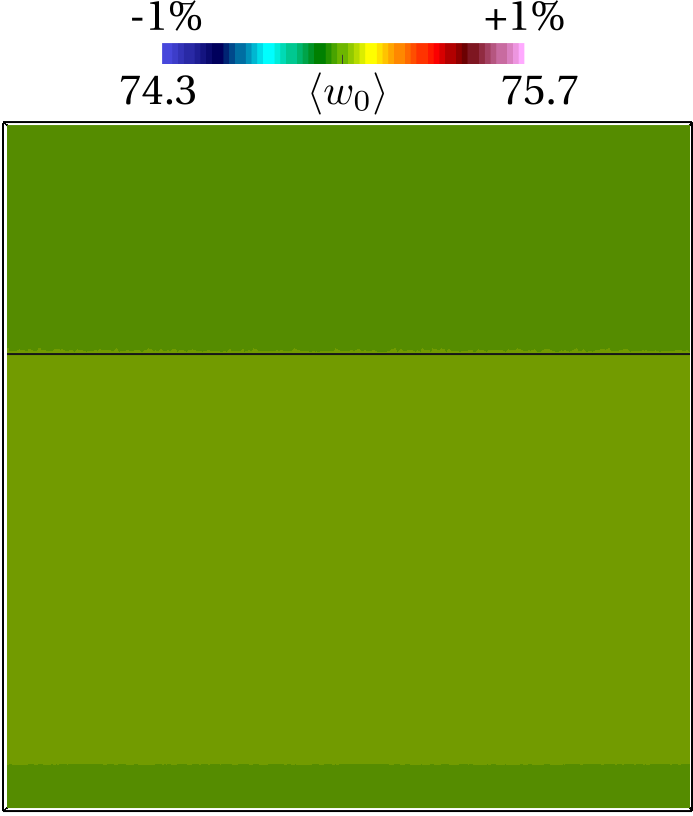
\includegraphics[width=\textwidth]{Chapter3/Graphics/freckle_fe/refA_new_annotate.png}
	\caption{FE-G1R1L0}
    \label{fig:refA}
  \end{subfigure}
   %------------------------------
  \vskip\baselineskip
  %------------------------------
  \begin{subfigure}{0.4\textwidth}
    \centering
	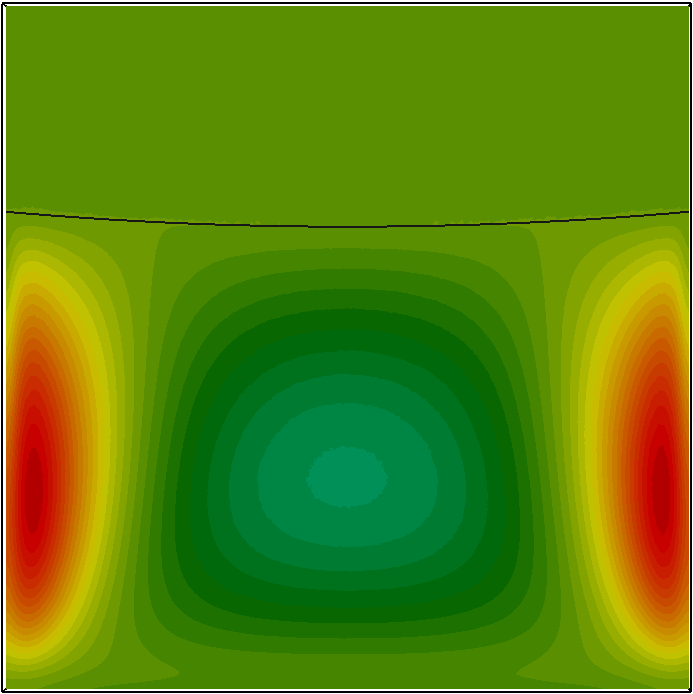
\includegraphics[width=\textwidth]{Chapter3/Graphics/freckle_fe/refB_new.png}
	\caption{FE-G1R1L1}
    \label{fig:refB}
  \end{subfigure}
   %-----------
  \vskip\baselineskip
  %------------------------------
  \begin{subfigure}{0.4\textwidth}
    \centering
	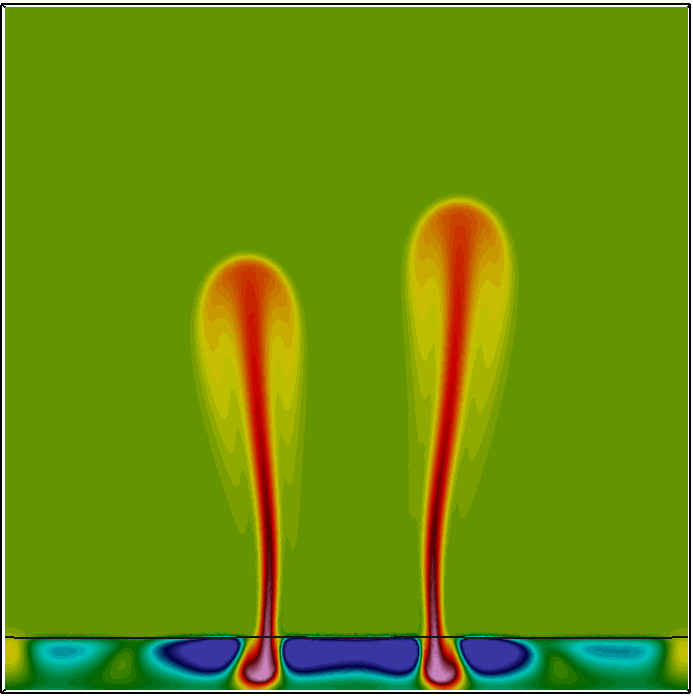
\includegraphics[width=\textwidth]{Chapter3/Graphics/freckle_fe/refC_new.png}
	\caption{FE-G2R1L1}
    \label{fig:refC}
  \end{subfigure}
   %------------
\caption{Average Ga composition field at \SI{250}{\utime} for the 3 FE cases showing the influence of 
process parameters on the freckling tendency. The black line represents the liquidus isotherm given in \cref{table:data_case_InGa}.} 
\label{fig:freckles_fe}
\end{figure}
%-----------------
%
\Cref{fig:planche_fe} gives a series of snapshots for case FE-G2R1L1 at three different times. Among the two clear distinct 
plumes that are visible at \SI{250}{\utime} in \cref{fig:freckles_fe}, only one has led to a channel formation,
that remains in \cref{fig:planche_fe} at \SI{500}{\utime}. 
In fact, an animation between \SI{250}{\utime} and \SI{500}{\utime} (not shown here) reveals that one plume vanishes, 
thus permitting the first one to further develop. A second freckle is also seen on the left hand side of the cell. 
These two freckles are stable for a long time since they remain at time \SI{1000}{\utime}. However, the left side freckle 
develops further to become the main one at \SI{1500}{\utime}, while the mid-width freckle decreases in intensity, changes 
orientation and subsequently disappears (not shown here). Thus, the birth and death of very few freckles is observed in this 
simulation, mainly due to solutal instability, as the temperature field shown in \cref{fig:planche_fe} clearly remains stable despite 
the low lateral heat flux. As shown in \cref{fig:freckles_fe}, instability is yet required to create these chemical plumes and channels. 
Here, it is created by a very small lateral heat flow but other sources of instability could be involved, as shown with the grain structure in the next section.
%
%=====================================BIG LANDSCAPE FIGURE =====================================
\begin{landscape}
\begin{figureth}
{1.15}
{Chapter3/Graphics/freckle_fe/planche_fe.pdf}
{Simulation results for case FE-G2R1L1 showing maps of the average composition in gallium,
the solid fraction, the superficial velocity field (vertical component) and the temperature, 
on a cut plane at the center of the cell at 500 s, 1000 s and 1500 s.}
\label{fig:planche_fe}
%\thispagestyle{headings}
\end{figureth}
\end{landscape}
%=====================================BIG LANDSCAPE FIGURE =====================================
%
\subsubsection{Discussion}
In \cref{sec:intro_freckle}, we have introduced some successful attempts of freckle predictions. 
The authors tackled the problem from an qualitative perspective. 
To our knowledge, the closest work to quantitative freckling analysis in solidification literature was done by \citet{ramirez_evaluation_2003}.
They attempted to draw a correlation (freckling criterion) between the process parameters and the occurrence of freckles, 
(without any size or shape constraints, i.e. any flow instability that may appear and form the smallest freckle is considered). 
To accomplish this, they took a number of experiments done independently by \citet{pollock_breakdown_1996} and \citet{auburtin_freckle_2000} 
where the casting parameters vary one at a time: casting speed (R), thermal gradient (G), angle ($\theta$) with respect to vertical 
orientation and nominal composition ($\avg{w_0}$), giving a database for 6 different superalloys. The experimental results were 
compared to a modified Rayleigh number that accounts for the various parameters. It allowed them to define a threshold for freckle 
formation in Nickel-base superalloys, as well as Pb-Sn alloys.
Other contributions by \citet{yuan_new_2012} (Pb-Sn alloy) and  \citet{karagadde_3-d_2014} (In-Ga alloy) relied on a Cellular Automata Finite Difference
(CAFD) model developed by \citet{lee_modeling_2002}, which  solves the dendrite tip growth kinetics at 
the solid-liquid interface together with macroscopic conservation equations. 
The authors compared the simulated formation of freckles with the results obtained by \citet{shevchenko_chimney_2013}.
However, these simulations follow solidification in a small volume that contains a few dendrites with interdendritic liquid, 
therefore limited as far as to predict the liquid behaviour outside the mushy zone.
On another hand, experimental observations reveal a great deal of information 
regarding solute redistribution, first in the chimneys that wash the dendrites in their 
way and then convective plumes that expel chemical species outside the mush, resulting in a global complex phenomenon.
In order to capture simultaneously the interaction between the mushy zone and the free liquid, we use 
the Cellular Automata Finite Element (CAFE) method to combine the macroscopic and mesoscopic length scales
and predict more realistic channel segregation.
%
%-----------------------------------------------
\section{Meso-Macro prediction of channel segregates}
%
\subsection{Numerical method}
%
\subsubsection{Microscopic scale}
The CAFE model introduces a grid of regular and structured cubic cells, with a constant size 
in all space directions, referred to as the cellular automaton (CA) grid. It is different from 
the unstructured finite element mesh previously mentioned for the solution of the average conservation 
equations. A typical CA step dimension is smaller than the smallest FE mesh size. The CA grid serves to 
represent solidification phenomena including nucleation, growth and remelting of the envelope of the 
primary dendritic grains. Details about the CAFE model can be found in \citep{carozzani_3d_2012,carozzani_direct_2013,carozzani_optimized_2014}. 
Cell information, such as the temperature, the average composition or the velocity of the liquid phase, is interpolated from 
the nodes of the FE mesh. State indices are also defined for each CA cell, providing the presence of liquid or solid phases. 
%
\subsubsection{Nucleation}
Initially, cells are in a fully liquid state. In the present situation, random nucleation sites are 
chosen based on a nucleation density, $n_\text{max}$ (expressed in surface density inverse \si{\per \uarea}), at the 
bottom surface of the geometry in contact with the cooler. Nucleation occurs in a cell only if the 
latter contains a nucleation site, and when the local undercooling of the cell reaches the critical 
nucleation undercooling given as input by a Gaussian distribution of mean undercooling $\Delta T_N$ with a 
standard deviation $\Delta T_\sigma$. The crystallographic orientation of each grain newly nucleated is also randomly 
chosen using values of the Euler angles to fully define the three rotations that transform the reference 
frame to the $\avg{100}$ directions that define the main growth axes of the dendrite trunks and arms. Grain 
selection is therefore solely controlled by growth competition.
%
\subsubsection{Growth}
Dendrite growth is driven by the chemical supersaturation $\Omega_\textbf{saturation}$, which is a 
dimensionless number proportional to the difference between the liquid composition at the dendrite 
tip and the melt composition far away from the tip. The higher the supersaturation, the faster the 
dendrite tip velocity. However, in the presence of a convective fluid, the chemical supersaturation 
is highly influenced by the intensity and the direction of the flow with respect to the growth direction 
of the dendrites. In the current model, convection is central in studying freckle formation. Therefore, 
the purely diffusive Ivantsov relation used to determine the Peclet number $Pe$ as function of the supersaturation, 
is replaced by a modified relation using a boundary layer correlation model that accounts for both the intensity 
and the misorientation of the liquid velocity with respect to the growth direction of the dendrites \citep{gandin_boundary_2003}. 
The main parameters for this growth kinetics models are the Gibbs Thomson coefficient, $\Gamma_{\text{GT}}$, and the diffusion 
coefficient for Ga in In, $\Dl$.
%
\subsubsection{Solidification path}
The CA model gives the presence of the grains in the liquid as well as its growth undercooling. 
For coupling with macroscopic scale modelling, the fraction of phases needs to be fed back to the 
FE model. This is now done by accounting for the information provided by the CA model. Thus, the 
fraction of solid is no longer the consequence of a simple conversion of the temperature and 
composition assuming thermodynamic equilibrium. It also includes the solidification delay due to 
the kinetics of the development of the grains as detailed elsewhere in the work of \citet{carozzani_direct_2013}.
%
\subsubsection{Numerical method}
Both the finite element mesh and the cellular automaton grid play a role in predicting freckles inasmuch as 
this type of defect originate from interplays between hydrodynamic instabilities on the scale of the dendrites 
and macroscopic flows defined by the geometry of the experimental cell \citep{shevchenko_chimney_2013}. One has to 
respect a small maximum FE mesh size, comparable to the dendrite arm spacing. With such an element size, composition gradients giving 
rise to solutal buoyancy forces can be captured. This limits consequently the CA cell size, as a minimum number 
of cells is required in each finite element. In the array of simulations that will be presented in the next section, 
the value of $\sdas$ was considered. We have chosen a fixed mesh element size of 2$\sdas$ and a CA cell size of $\sdas/2$. 
An average of 4 CA cells per unit length of a finite element is enough to accurately compute the development of the 
grain envelopes together with the solutal, thermal and mechanical interactions.
%--------------------
%
\subsection{Configuration}
%----------------
%
%--------------------------------
\begin{table}
\centering
\caption{Summary of the simulations and and the corresponding parameters for the CAFE cases, coupling macroscopic model with the grain structure model.
Parameters are varied from (G1) low to (G2) high gradient, (R1) low to (R2) high cooling 
rate and (L0) no, (L1) low and (L2) high lateral cooling.}
\label{table:simulation_InGa_cafe}
\resizebox{\columnwidth}{!}{%
{\tabulinesep=1.1mm \begin{tabu}{C{3cm} C{3cm} C{3cm} C{3.0cm} C{3.5cm} C{3.2cm}}
\tabucline[1pt]{-}
\textbf{Case}  & Vertical gradient & Cooling rate & Lateral cooling & Initial temperature  & Nucleation  \\
			  &     G 			  & 	R		 & 			L \quad ($\hext$, $\Text$)	& ($T_{top}$, $T_{bottom}$) & ($n_\text{max}$, $\Delta T_N$, $\Delta T_\sigma$) \\
 			  & [\si{\ugradT}] & [\si{\uCR}] & [\si{\uhconvec}, \si{\udegC}] & [\si{\udegC}] & [\si{\per \uarea}, \si{\udegC}, \si{\udegC}] \\\tabucline[1pt]{-}
%-----------------------------
CAFE-G2R1L1  & G2:1.5 & R1:-0.01 & L1:(20,0) & (58.25, 25.25)  & (\num{e6}, 1, \num{0.2}) \\ 
CAFE-G1R1L1  & G1:0.2 & R1:-0.01 & L1:(20,0) & (29.75, 25.25)  & (\num{e6}, 1, \num{0.2}) \\ 
CAFE-G1R1L2  & G1:0.2 & R1:-0.01 & L2:(500,0) & (29.75, 25.25) & (\num{e6}, 1, \num{0.2}) \\ 
CAFE-G2R2L1  & G1:0.2 & R2:-0.05 & L1:(20,0) & (29.75, 25.25)  & (\num{e6}, 1, \num{0.2}) \\\tabucline[1pt]{-}
%-----------------------------
\end{tabu}}
}
\end{table}
%--------------------------------
%
%=====================================BIG LANDSCAPE FIGURE =====================================
\begin{landscape}
\begin{figureth}
{1.15}
{Chapter3/Graphics/freckle_cafe/planche_cafe.pdf}
{Simulation results for case CAFE-G2R1L1 showing maps of the average composition in gallium,
the solid fraction, the superficial velocity field (vertical component) and the temperature, 
on a cut plane at the center of the cell at 500 s, 1000 s and 1500 s.}
\label{fig:planche_cafe}
%\thispagestyle{headings}
\end{figureth}
\end{landscape}
%=====================================BIG LANDSCAPE FIGURE =====================================
%
%-----------------------
\begin{figureth}
{0.6}
{Chapter3/Graphics/freckle_cafe/planche_composition_grain.pdf}
{Simulation results the predicted of mushy grain structure with the corresponding composition maps.}
\label{fig:planche_composition_grain}
\end{figureth}
%-----------------------
%
Knowing that the configuration in FE-G2R1L1 produces segregated channels, the same set of parameters is first used 
for case CAFE-G2R1L1 by adding the effect of the grain structure using the CAFE model. Results are accessible 
in \cref{fig:planche_cafe} for comparison with \cref{fig:planche_fe}. A striking difference is seen: the composition maps become more 
perturbed as shown by the formation of numerous plumes when coupling with grain structure is active. The growing 
front displayed on the grain structure at the right most column of \cref{fig:planche_cafe} dictates the leading position of the 
mushy zone shown in the third column. Note that each color corresponds to one grain, with 17 grains having nucleated 
at the cell’s bottom surface. However, comparison of the solid fraction maps between \cref{fig:planche_fe} and \cref{fig:planche_cafe} at the 
same times reveals a delay in the growing front position. Values of the nucleation parameters in \cref{table:simulation_InGa_cafe} are such 
that few grains rapidly form below the nominal liquidus isotherm. The delay is therefore not due to the nucleation 
undercooling but to the growth undercooling of the dendrite tips. It should be noticed that, the growth front driven 
by undercooling in \cref{fig:planche_cafe} also forms with a higher initial solid fraction and hence larger solute segregation occurs 
at the front. This effect, together with instabilities of the composition field, is caused by a more perturbed fluid flow 
and more plumes as observed in CAFE-G2R1L1 compared to FE-G2R1L1. Such observations fit to the complicated fluid and solute 
flow patterns typically occurring in the experiments as shown in \cref{fig:experimental_freckles_gradients}. It becomes obvious that the consideration of grain 
structure and growth undercooling are vital to accurately simulate segregated channels formation in these experiments. The reasons for the 
instabilities are discussed hereinafter. In the present 3D CAFE simulation, each grain shown in \cref{fig:planche_composition_grain} 
is associated with a crystallographic orientation. 
The growth kinetics is only given for the $\avg{100}$ crystallographic directions at the grain boundaries with the liquid. The CA growth model 
is based on the hypothesis that, in a quiescent liquid of uniform temperature distribution and composition, the grain envelop should 
reproduce an octahedral grain shape with main directions given by the six $\avg{100}$ directions. In the present situation where complicated 
fields are present for temperature, composition and liquid velocity, each grain envelope with different crystallographic orientation 
adapts differently to its local environment. Thus, the local undercooling of the front varies everywhere. Such variations are within 
few degrees here, but this is sufficient to create irregularities on the growth front, as seen on the grain structure in \cref{fig:planche_composition_grain}. 
Apart from that, these variations are linked to the position of the instabilities for the chemical and liquid velocity fields, thus 
demonstrating the full coupling between the CA and FE models.
%
%
%-----------------
\begin{figure}[htbp]
\centering
  %------------
  \begin{subfigure}{0.4\textwidth}
    \centering
	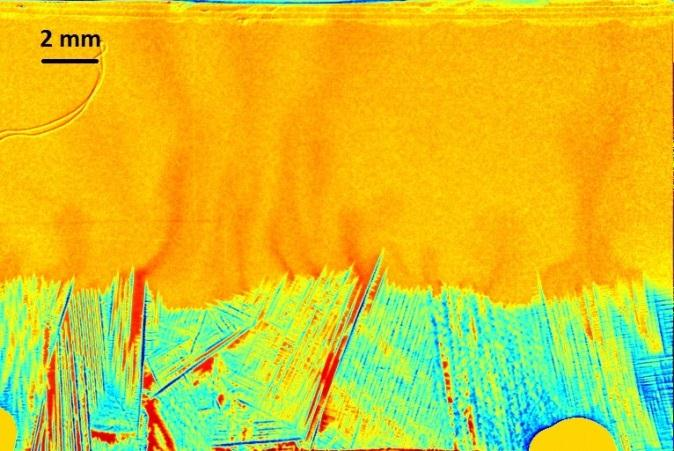
\includegraphics[width=\textwidth]{Chapter3/Graphics/freckle_exp/lowgrad.png}
	\caption{}
    \label{fig:exp_lowgrad}
  \end{subfigure}
   %------------------------------
  %\vskip\baselineskip
  %------------------------------
  \begin{subfigure}{0.4\textwidth}
    \centering
	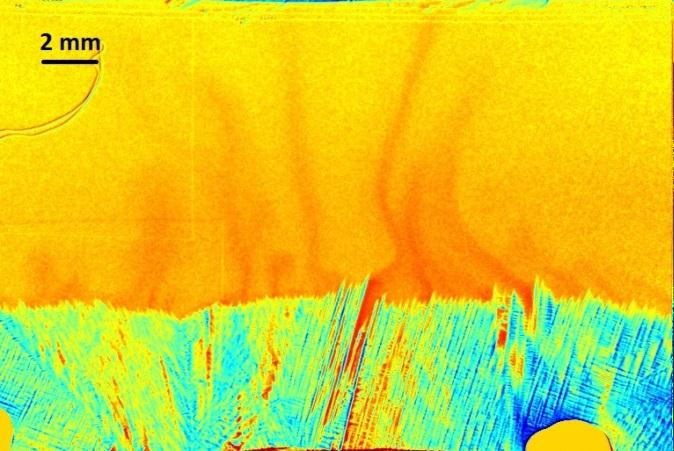
\includegraphics[width=\textwidth]{Chapter3/Graphics/freckle_exp/highgrad.png}
	\caption{}
    \label{fig:exp_highgrad}
  \end{subfigure}
   %------------
\caption{Snapshots of dendritic structure and composition field 
obtained from two solidification experiments at a cooling rate 
R=\SI{-0.01}{\uCR} and temperature gradients of (a) G=\SI{1.1}{\ugradT} and (b) G=\SI{1.3}{\ugradT}} 
\label{fig:experimental_freckles_gradients}
\end{figure}
%-----------------
%
%
\subsection{Effect of vertical temperature gradient}
The influence of diverse process parameters can now be considered in context of the grain structure. 
The effect of the vertical temperature gradient is shown by comparing the previous case CAFE-G2R1L1 
with case CAFE-G1R1L1. The temperature gradient is decreased about 7 times here, from G2=\SI{1.5}{\ugradT}
to G1=\SI{0.2}{\ugradT}. In fact, both cases share almost all traits with respect to flow patterns and velocity
magnitude in the bulk. Main differences are yet seen regarding the dynamics of the plumes shown in 
\cref{fig:cafe_G1G2}. In the case of a low temperature gradient (G1), the solidification front cannot maintain a 
shape as smooth as for the case of a large temperature gradient (G2): the solute gradient in the 
liquid of the mushy zone (basically following the lever rule approximation for a given temperature) 
decreases, leading to a lower gradient of the solutal buoyancy force. In turn, more solute accumulates 
close to the front and locally reduces the growth velocity, thus creating larger “valleys” or steps 
with higher solute content. The irregular geometry of the front is also influenced by the dendrite tip 
growth kinetics model. The velocity of the isotherms is the ratio of the cooling rate, R, to the 
temperature gradient, G. Consequently, the isotherm velocity in case G1 is larger than in G2, since 
cooling rate, R1, is the same in both cases. Moreover, because the dendrite tip velocity is a monotonously 
increasing function with the undercooling \citep{gandin_boundary_2003}, the latter for CAFE-G1R1L1 is larger 
than for CAFE-G2R1L1. Height differences of the growth front are proportional to the variations of the 
undercooling by the temperature gradient. Therefore, this forms larger steps on the growth front for case 
G1 compared to G2. The chimney extends deeper in the mushy zone when the temperature gradient increases. 
This is confirmed by both the simulation results shown in \cref{fig:cafe_G1G2} as well as the experimental observations. 
Another remarkable phenomenon is also observed in the low gradient case: a “pulsing” mechanism in CAFE-G1R1L1 
where a series of solute rich liquid pockets are observed one above the other. This corresponds to a repeated
and localized strong spatial variation of the liquid velocity field outside the mushy zone, regularly thrusting 
away small plumes. These pulses are roughly similar to each other in size and exit speed, creating thus a very 
regular pattern during some time. 
%
%-----------------
\begin{figure}[htbp]
\centering
  %------------
  \begin{subfigure}{0.4\textwidth}
    \centering
	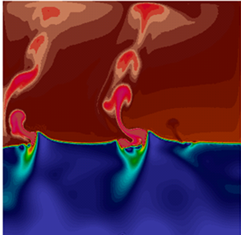
\includegraphics[height=5cm]{Chapter3/Graphics/freckle_cafe/cafe_VG1_composition.png}
	\caption{}
    \label{fig:cafe_VG1}
  \end{subfigure}
  %\hfill
  \begin{subfigure}{0.01\textwidth}
    \centering
	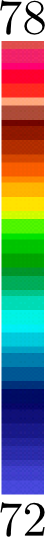
\includegraphics[height=5cm]{Chapter3/Graphics/freckle_cafe/cafe_VG_colorbar_annot.png}
	%\caption{}
    \label{} % Do not delete or comment this line to preserve alignment
  \end{subfigure}
  \hspace{2mm}
   \begin{subfigure}{0.4\textwidth}
    \centering
	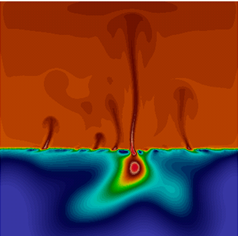
\includegraphics[height=5cm]{Chapter3/Graphics/freckle_cafe/cafe_VG2_composition.png}
	\caption{}
    \label{fig:cafe_VG2}
  \end{subfigure}
   %------------
\caption{Average composition maps for CAFE-G1R1L1 at time 1060 s and CAFE-G2R1L1 at time 1845 s.} 
\label{fig:cafe_G1G2}
\end{figure}
%-----------------
%
%=====================================ANIMATION FIGURE =====================================
\begin{figure}[htbp]
\centering
%\animategraphics[options]{fps}{filename_without_number}{1}{N}
%-------
 \animategraphics{10}{Chapter3/Graphics/freckle_cafe/anim_pulsing/img}{1}{11}
%-------
\caption{Animation of the pusling mechanism coming from a groove shape in the mushy.} 
\label{fig:animate_cafeVG1}
\end{figure}
%=====================================ANIMATION FIGURE =====================================
%
In the case of a high temperature gradient (case CAFE-G2R1L1) this phenomenon is 
barely seen. In fact, the pattern shown in \cref{fig:cafe_G1G2} is more typical, with continuous plume rising from the mushy 
zone and reaching the top of the domain. However, such regular plume is the initial and final pattern seen for low 
gradient before the pulsing regime. Similar observations have been made in the experiments too. \Cref{fig:exp_pulsing} displays 
the phenomenon of the “pulsing” plumes, which could be explained by the following mechanisms. The permeability of the 
mushy zone and the narrow gap of the solidification cell obstruct the feeding of the plumes by solute. A critical solute 
concentration has to be accumulated at a specific location in order to trigger the formation of a rising plume. An interim 
drop of the solute concentration below such a threshold would interrupt the plume. Flow instabilities can be another reason 
for the peculiar shape of the plumes. \Cref{fig:exp_continuous} shows a pronounced continuous plume. The same plume can be seen a few seconds 
later in \cref{fig:exp_instability}. The plume structure becomes unstable; one can observe an indentation of streamlines followed by a mixing of 
rising solute-rich liquid with descending In-rich fluid. This mechanism also causes a non-continuous structure of the plumes.
%
%-----------------
\begin{figure}[htbp]
\centering
  %------------
  \begin{subfigure}{0.3\textwidth}
    \centering
	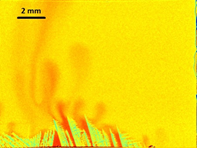
\includegraphics[width=\textwidth]{Chapter3/Graphics/freckle_exp/exp_pulsing.png}
	\caption{}
    \label{fig:exp_pulsing}
  \end{subfigure}
   %----------------
  \begin{subfigure}{0.3\textwidth}
    \centering
	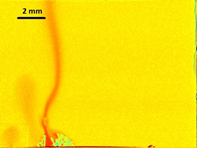
\includegraphics[width=\textwidth]{Chapter3/Graphics/freckle_exp/exp_continuous.png}
	\caption{}
    \label{fig:exp_continuous}
  \end{subfigure}
   %------------
   \begin{subfigure}{0.3\textwidth}
    \centering
	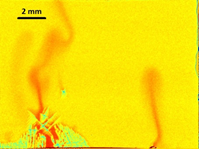
\includegraphics[width=\textwidth]{Chapter3/Graphics/freckle_exp/exp_instability.png}
	\caption{}
    \label{fig:exp_instability}
  \end{subfigure}
   %------------
\caption{Snapshots of dendrite structure and composition field from two 
solidification experiments conducted at a cooling rate 
R=\SI{-0.01}{\uCR} and a temperature gradient =\SI{1}{\ugradT}: (a) “pulsing” plumes, 
(b) continuous plume, (c) upcoming plume instability.} 
\label{fig:experimental_freckles_regimes}
\end{figure}
%-----------------
%
%
\subsection{Effect of cooling rate}
The next parameter studied is the cooling rate, corresponding to case CAFE-G1R2L1. A snapshot of the composition map 
and the corresponding vertical component of the velocity field are given in \cref{fig:cafe_R1R2}. We see a similarity 
with case CAFE-G1R1L1 in \cref{fig:cafe_VG1} with respect to the buckled interface between the liquid and the mushy 
zone as well a plume pulsing effect when a low temperature gradient is applied. On the other hand, segregation inside 
the mush is more irregular with more pronounced patterns reaching a larger depth. One could distinguish alternating V  
and A shapes patterns in the mushy zone. As for case CAFE-G1R1L1, these patterns are created by a network of pulsing 
plumes formed by the steps created on the delocalized growth front due to the low temperature gradient. However, these 
considerations are not sufficient to explain the shape of the growth front. The reason for the protuberances created at 
the tips of the V shape is the presence of a descending bulk liquid with a low composition seen by the growth front. It 
infers that favorable growth conditions are created for a higher working temperature since the dendrite tip undercooling 
decreases for facing liquid flow and a lower composition; the growth rate is given by the isotherm velocity. The growth 
front thus adjusts its position to catch up with the corresponding isotherm, the latter being located at the tips of the 
V shape, i.e. the outmost advanced position of the growth front. It also means that the V shape angle depends on the size 
and intensity of the convection loops above the front. When the steps are formed on the growth front, the plumes exiting 
the mushy zone follow a direction normal to the front. They are inclined towards each other above the V shape. As a result, 
they may join and form a larger plume as seen in CAFE-G1R1L1 (\cref{fig:cafe_VG1}), thus forming larger and more stable segregated channels. 
The other observation in \cref{fig:cafe_R1R2} is the existence of stable regions of the growth front. For instance, this is seen 
in between the two V shape forming or on the right hand side of the cell. 
%
%-----------------------
\begin{figureth}
{0.8}
{Chapter3/Graphics/freckle_cafe/planche_CR.pdf}
{Average fields inside the cell for case CAFE-G1R2L1 at 350 s. 
The white contour identifies the zero velocity limit for the vertical component of the velocity field}
\label{fig:cafe_R1R2}
\end{figureth}
%-----------------------
%
The reason for this stability is the inversion of 
the composition gradient located ahead. Animation shows that solute coming from the top of the cell is responsible for this 
accumulation, creating a layering that provides a stabilization effect above the mushy zone. This is verified by the vertical 
component of the average velocity also made available in \cref{fig:cafe_R1R2}. It is negative outside the path of the plumes. A resulting 
concurrent effect is the formation of the A shape segregates in between the V shape patterns seen in \cref{fig:cafe_R1R2}. Finally, it can 
be observed that these patterns are sustained longer compared to \cref{fig:cafe_G1G2} CAFE-G1R1L1 because, at high cooling rate, 
the flow in the mushy zone is decreased due to a faster solidification. This is the same effect as described for the large gradient 
configuration in CAFE-G2R1L1 (\cref{fig:cafe_VG2}).
It is not clear how these observations could be compared with the A  and V  shapes segregates reported for steel ingots 
\citep{pickering_macrosegregation_2013}. Despite the fact that macrosegregation is the main phenomenon leading to these 
patterns, there has not been a clear explanation yet in the literature for their formation. However, for steel casting, 
the A and V patterns are believed to form concomitantly. Further investigations would thus be required to quantify the 
consequences of thermosolutal instabilities simulated here for an \bin{In}{75}{Ga} alloy and check their possible correlation 
with experimental observations in steel casting.
%
\subsection{Effect of lateral temperature gradient}
The previous simulations show the effect of cooling rate and temperature gradient on the survival of segregation patterns deep 
in the mushy zone. Another simulation is performed by increasing the cooling rate using higher heat flux extracted from the 
vertical side boundaries. This is achieved in case CAFE-G1R1L2 where the heat transfer coefficient reaches \SI{500}{\uhconvec}. 
As a consequence of the large cooling from the sides, the temperature gradient is no longer vertical. A distinct flow due to 
thermal buoyancy is created, driving a cold liquid downwards near the sides of the cell. Under the influence of these 2 main 
convection loops, all segregation plumes tend to regroup in the middle of the domain, forming a larger central plume, as seen in 
the composition map at 450 s in \cref{fig:planche_LG}. However, this regime occurs at times earlier than 500 s, where the effect of thermally 
induced buoyancy forces is prevailing, feeding the convection loops. Approximately 500 s later, the mushy zone has extended, favoring 
the segregation mechanical forces i.e.  $\rhoref \brac{1-\betawl \Delta \wl} \gravity$, rather than the thermal mechanical forces, $\rhoref \brac{1-\betaT \Delta T} \gravity$. 
%
%-----------------------
\begin{figureth}
{1.0}
{Chapter3/Graphics/freckle_cafe/planche_LG.pdf}
{2D cut plane of the average composition inside the cell for case CAFE-G1R1L2 at the 
following time increments: 450 s, 1000 s and 1500 s.}
\label{fig:planche_LG}
\end{figureth}
%-----------------------
%
\Cref{fig:planche_LG} shows the corresponding composition maps with stable chimneys at about 1000 s that also remain at 1500 s. The solidification 
front then tends to form a concave shape at the center of the cell, thus partially revealing the form of the isotherms toward the cell 
center. The stable pattern in the center is similar to the plateau seen at the center, between the A-shapes in \cref{fig:cafe_G1G2} and \cref{fig:cafe_R1R2}. 
As stated before, it is an inactive region with respect to plume initiation due to the inversion of the solute composition gradient.
In other words, the high gallium concentration at the top of cell causes indium, which is the heavier species, to accumulate and be partially 
trapped between the mushy walls, thus creating a stable flow configuration.
Outside of the plateau, 2 plumes are observed from the prominent instabilities of the growth front, adopting diverging directions. 
This is also observed at the center of the cell in \cref{fig:cafe_R1R2} on each side of the A-shape segregate. 
These plumes in \cref{fig:planche_LG} lead to the formation of two stable channels. 
The corresponding situation in the experiment is shown in \cref{fig:exp_G1R1}. The chimneys on both sides and the plateau in between can be clearly 
recognised. The additional cooling at the side walls produces two flow vortices between the side wall and the strong convective plumes above the 
chimneys. The central part of the sample remains almost unaffected by the additionally driven thermal convection. This area is characterised by 
the occurrence of a number of smaller convective plumes.  
%
%-----------------------
\begin{figureth}
{0.6}
{Chapter3/Graphics/freckle_exp/exp_G1R1.png}
{Snapshot of dendritic structure and composition field from a 
solidification experiment recorded at 1000 s for a cooling rate R=\SI{-0.01}{\uCR} and a temperature gradient G=\SI{-1}{\ugradT}.}
\label{fig:exp_G1R1}
\end{figureth}
%-----------------------
%
\subsection{Mono-grain freckles}
All CAFE simulations were performed considering a normal classic heterogeneous nucleation at 
the surface of the mould where the metal is cooled down. However, as the number of grains is
not negligible, the subsequent fluid-structure interaction between dendrites, simply represented by an isotropic permeability 
and the interdendritic flow cannot be easily interpreted. Therefore, one may consider simpler solidification cases 
like a mono-grain growth. This ideal situation is not always experimentally viable: either the mould surface is not 
perfectly smooth, and therefore nucleation can be triggered by a wetting mechanism, or the metal contains a certain level of impurity
which can trigger nucleation heterogeneously in the liquid bulk. 
Regardless of this experimental limitation, this type of simulations allows simpler understanding as the grain growth is not 
disturbed by another neighbouring grain, it grows while exclusively interacting with the liquid phase.
%
%===================================== ANIMATION FIGURE =====================================
% \begin{figure}[htbp]
% \centering
  ------------
  % \begin{subfigure}{0.45\textwidth}
	% \centering
	% \animage{height=6cm}{6}{Chapter3/Graphics/freckle_cafe/anim_monograin_upright/img0}{030}{133}{.png} % 0000 to 0139
	% \caption{}
    % \label{fig:mono_upright}
  % \end{subfigure}  
  ------------
	% \hfill %\hspace{1mm}  
	 % \begin{subfigure}{0.05\textwidth}
	% \centering
	% 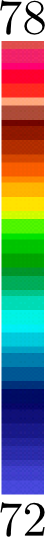
\includegraphics[height=6cm]{Chapter3/Graphics/freckle_cafe/cafe_VG_colorbar_annot.png}
	% \caption{}
    % \label{} % Do not delete or comment this line to preserve alignment
  % \end{subfigure}
	% \hfill %\hspace{1mm}  
  ------------
  % \begin{subfigure}{0.45\textwidth}
    % \centering
    % \animage{height=6cm}{6}{Chapter3/Graphics/freckle_cafe/anim_monograin_tilted/img0}{030}{133}{.png} % 0000 to 0133
	% \caption{}
    % \label{fig:mono_tilted}
  % \end{subfigure}
-------
% \caption{Animations of mono-grain solidification showing the average composition in gallium predicted by the CAFE approach. 
% Two orientation scenarios are considered where a) the grain is upright with a Euler angle of \orient{90}{0}{0} 
% or b) the grain is tilted with a Euler angle of \orient{90}{30}{0}.}
% \label{fig:animate_monograin}
% \end{figure}
%===================================== ANIMATION FIGURE =====================================
%
%=====================================ANIMATION FIGURE shared control buttons ===================================
%
%-----------------------
\begin{figure}[htbp]
\centering %
\begin{animateinline}{6}%
 %\multiframe{nb_frames}{i=start_nb+inc_nb}{%
  \multiframe{108}{i=25+1}{%
  		
      \includegraphics[height=6cm]{Chapter3/Graphics/freckle_cafe/anim_monograin_upright/img\zeropad{1234}{\i}.png}%
	  \hspace{1mm}%
      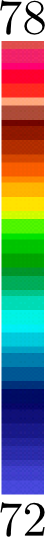
\includegraphics[height=6cm]{Chapter3/Graphics/freckle_cafe/cafe_VG_colorbar_annot.png}%
	  \hspace{1mm}%      
      \includegraphics[height=6cm]{Chapter3/Graphics/freckle_cafe/anim_monograin_tilted/img\zeropad{1234}{\i}.png}%
  }%
\end{animateinline}%
\caption{Animations of mono-grain solidification showing the average composition in gallium predicted by the CAFE approach. 
 		Two orientation scenarios are considered where a) the grain is upright with a Euler angle of \orient{90}{0}{0} 
 		or b) the grain is tilted with a Euler angle of \orient{90}{30}{0}.}
\label{fig:animate_monograin}
\end{figure}
%=====================================ANIMATION FIGURE =====================================
